\chapter{The event generation procedure}
\label{sect:gen_proc}
\section{Event generation with weights}
\label{sect:gen_with_weights}
%Phase space distributions and weights.
%Phase space plots: $W$ vs $Q^{2}$ and Dalitz plots.
%Refer to the Bycling Caianti.

%Note that uncertainties of the efficiency are calculated differently (ref. to Sacle note).

%---------------------------------------------

For this EG the method of generation with weights is used. It means that instead of forcing the number of generated events in particular kinematical point to be proportional to the cross section value at this point, the number of generated events is maintained the same everywhere, while each event acquires an individual weight that is equal to that cross section value. In this way the generated events still reproduce the realistic cross section shape if they are summed up with weights.

The weight for each event is calculated based on the model structure functions in the ($W$, $Q^2$) regions, where experimental data exists. In other areas, where no experimental data exists, the weight is estimated based on a special procedure of interpolation and extrapolation of the structure functions from the areas covered with data (see Sect.~\ref{sect:data} for details). 


As it is mentioned in Sect.~\ref{sect:cr_sect_model} the model structure functions are differential in the following kinematical variables ($S_{12}$, $S_{23}$, $(-cos\theta_{\pi^{-}})$, $\varphi_{\pi^{-}}$, $\alpha_{\pi^{-}}$) and given for different ($W$, $Q^2$) points for the variable set, where $\pi^{-}$ is assumed to be the first particle. This forces us to use this framework for the event generation. 

Below all subscript indices $1,\;2,\;3$ correspond to the final hadron numbering, which is in the second set of variables the following: $1st\; - \pi^{-},\; 2nd \; - \pi^{+},\;3rd - p'$. The subscript index $h$ corresponds to $hadron$ and in the second set of variables it is $\pi^{-}$.

For each event the values of all kinematical variables $W$, $Q^2$, $S_{12}$, $S_{23}$, $cos \theta_{h}$, $\phi_{h}$, $\alpha_{h}$ are generated randomly~\footnote[1]{If you use ROOT functions, it is convenient to use random number generator class TRandom3. \\
TRandom3 rndm\_name(UInt\_t(((float) rand() / (float)(RAND\_MAX))*4000000000.)); \\
Var =rndm\_name.Uniform(var\_min,var\_max); \\
It is convenient to use separate random generators for each variable that needs to be generated randomly. It is essential because if the same random generator is used for all variables, the generation constrains (discussed in the text under 1. and 2.) may disturb the randomnicity of the generation of some variables.} according to the double pion production phase space. This means that:
% refer to the root TRandom3 

\begin{figure}[htp]
\begin{center}
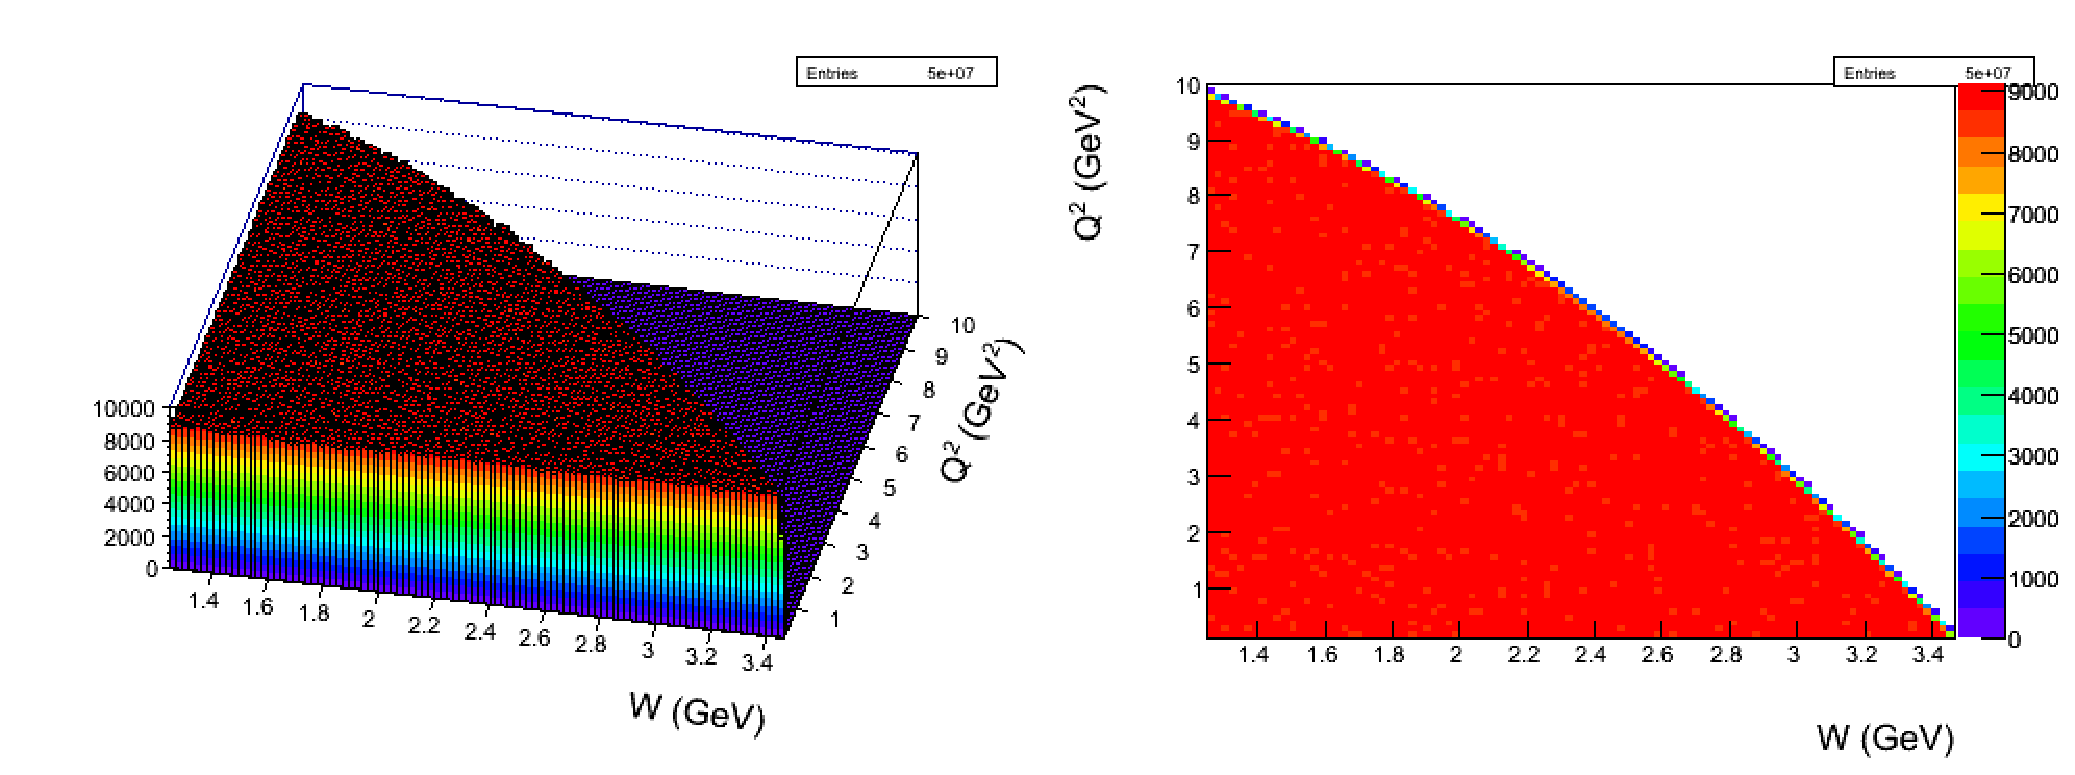
\includegraphics[width=16cm]{pictures/gen_proced/flat_w_vs_q2.pdf}
\caption{\small Generated flat $Q^2$ versus $W$ distribution for $E_{beam} = 6$ GeV. Left plot -- {\it lego2} option, right plot -- {\it  colz} option.   } \label{fig:w_vs_q2_flat}
\end{center}
\end{figure}

\begin{enumerate}
\item $W$ and $Q^2$ are generated flat in two-dimensional sense within the limits $[W_{min},W_{max}]$, $[Q^2_{min},Q^2_{max}]$, which are among the input parameters. Figure~\ref{fig:w_vs_q2_flat} shows an example of a $Q^2$ versus $W$ distribution. The triangle-like shape of this distribution is the consequence of the following constrain: $\nu < E_{beam} - E_{min}$, where $E_{beam}$ is the energy of the incoming electron beam and $E_{min}$ is the minimal energy of the scattered electron, respectively (both of them are defined in the lab frame and given as input parameters). This condition forces the energy of the virtual photon in the lab frame ($\nu$) to have reasonable values.

\item $S_{12}$ and $S_{23}$ are generated flat in two-dimensional sense within the limits $[(m_{1}+m_{2})^{2}, (W-m_{3})^2]$, $[(m_{2}+m_{3})^{2}, (W-m_{1})^2]$, where $W$ is the $W$-value generated in the previous step, $m_{1}$, $m_{2}$, and $m_{3}$ are the masses of the first, second, and third hadron, respectively. Figure~\ref{fig:s23_vs_s12_flat} shows an example of $S_{23}$ versus $S_{12}$ distribution. The shape of this distribution is determined by the condition $B(S_{12},S_{23},W^{2},m_{2}^{2},m_{1}^{2},m_{3}^{2}) <0$, where $B(x,y,z,u,v,w)$ is the Byckling function that is defined in the following way~\cite{Byckling:1971vca}:

\begin{equation}
\begin{split}
B(x,y,z,u,v,w) = &x^{2}y+xy^{2}+z^{2}u+zu^{2}+v^{2}w+vw^{2}+ \\   
&xzw+xuv+yzv+yuw- xy(z+u+v+w)- \\ 
&zu(x+y+v+w)-vw(x+y+z+u).
\label{eq:byckling}
\end{split}
\end{equation}

\item  $cos \theta_{h}$ is generated flat in a one-dimensional sense in the limits $[-1,~1]$. 
\item The angles $\varphi_{h}$ and $\alpha_{h}$ are generated flat in a one-dimensional sense in the limits $[0,~2\pi]$.
\end{enumerate}




\begin{figure}[htp]
\begin{center}
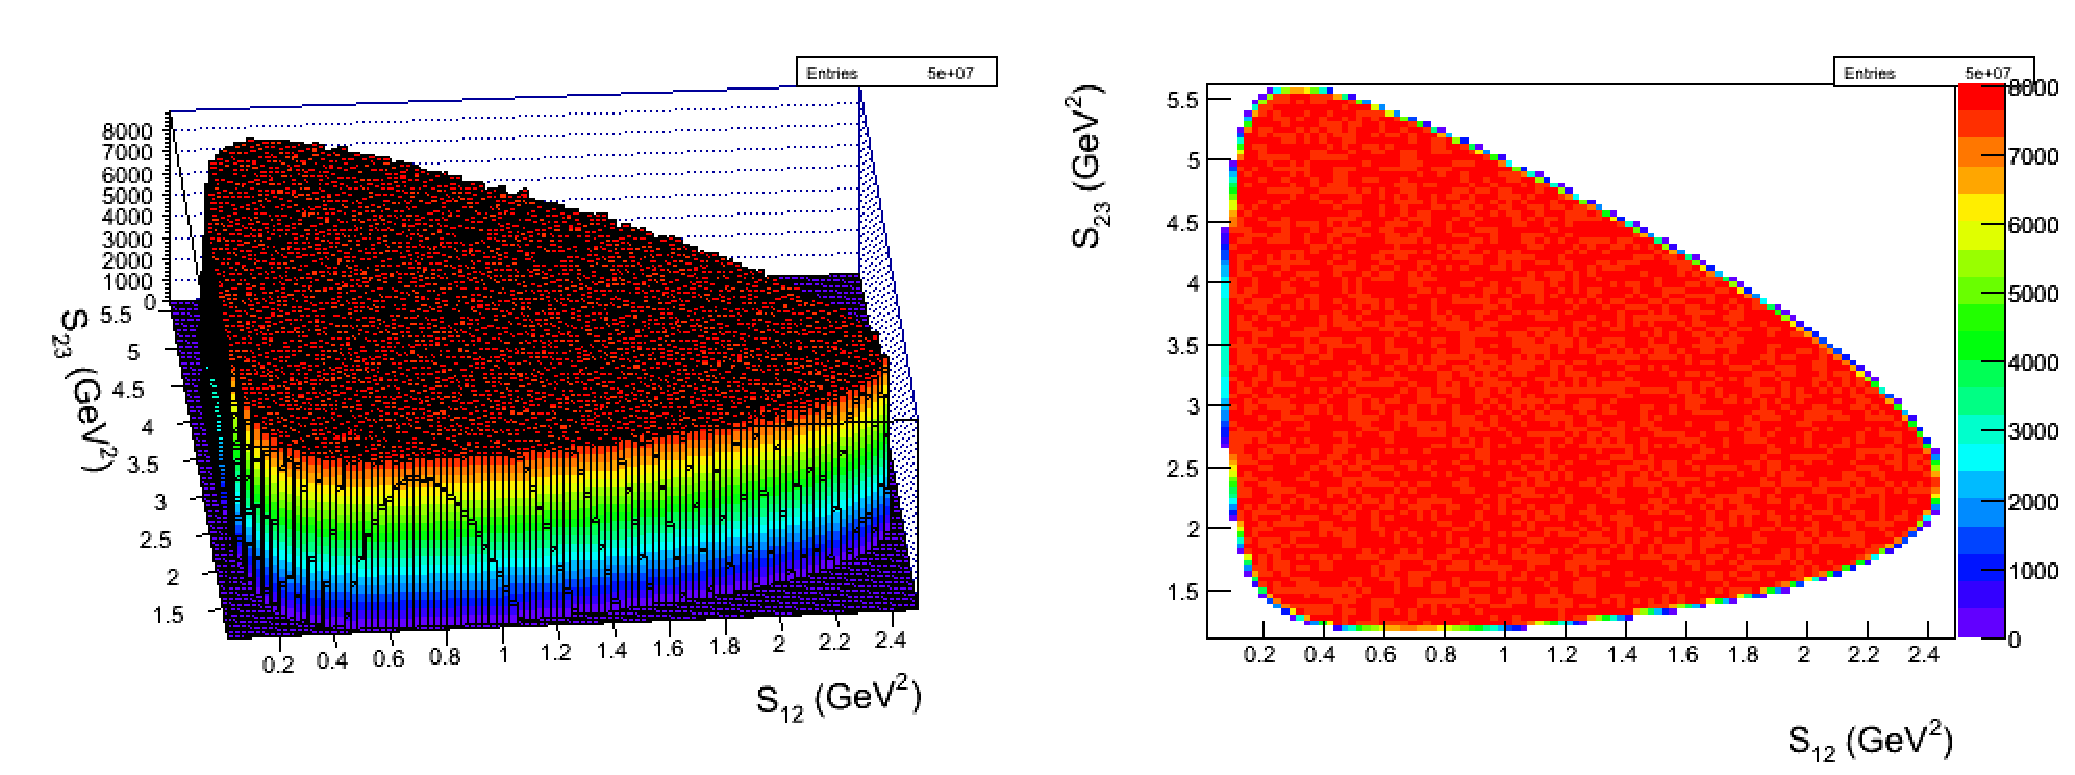
\includegraphics[width=16cm]{pictures/gen_proced/flat_s23_vs_s12.pdf}
\caption{\small Generated phase space $S_{23}$ versus $S_{12}$ distribution for  $W = 2.5$ GeV.  Left plot -- {\it lego2} option, right plot -- {\it  colz} option.  } \label{fig:s23_vs_s12_flat}
\end{center}
\end{figure}


Note that those variables must be generated flat in which the model cross section is differential. It is essential for the correct weight propagation.

All generated variables listed above are assumed to be defined in the CMS. 

Furthermore, the azimuthal angle of the scattered electron in the lab frame $\varphi_{e'}$ and its $z$-vertex $Z_{e'}$ are generated flat in a one-dimensional sense in the limits $[0,~2\pi]$ and $[Z^{off}_{targ}  - L_{targ}/2,~Z^{off}_{targ}  + L_{targ}/2]$, respectively, where $Z^{off}_{targ}$ and $L_{targ}$ are among the input parameters.

It also needs to be mentioned that if one uses a weighted EG for the purpose of efficiency evaluation, the statistical uncertainty of the efficiency must be calculated in a slightly different manner compared to the unweighted case. The proper way to calculate the uncertainty is discussed in~\cite{Laforge:1996ts}. 


\section{Obtaining particle four-momenta in the lab frame}
\label{sect:cms_to_lab_trans}
%According to the code.

%All kinematical variables discussed in the previous section are assumed to be generated in the CMS (if frame-dependent). 
The final goal of the event generation process is the following: using the generated values of all kinematic variables described in the previous section, to obtain the four-momenta of all final particles in the lab frame. All frame-dependent kinematic variables (angles) are assumed to be generated in the CMS.

The lab frame corresponds to the system, where the target proton is at rest and the axis orientation is the following: $Z_{lab}$ -- along the beam, $Y_{lab}$ -- up, and $X_{lab}$ -- perpendicular to the $YZ$-plane.

%The CMS frame has the following axis orientation: $Z_{cms}$ -- along the virtual photon, $X_{cms}$ --- in electron scattering plane $(e,e')$, $Y_{cms}$ -- perpendicular to the $XZ$-plane.

For the scattered electron the task is rather straightforward. Its four-momentum can be calculated in the lab frame in the following way,

\begin{equation}
\begin{split}
  \nu &= \frac{W^2+Q^2-m_{p}^{2}}{2m_{p}}\\
  E_{e'} &= E_{beam}-\nu\\
 \theta_{e'} &= acos\left (1-\frac{Q^2}{2E_{beam}E_{e'}}\right )\\
P_{e'}^{4} = (E_{e'}sin \theta_{e'}cos \varphi_{e'}&,E_{e'}sin \theta_{e'}sin \varphi_{e'},E_{e'}cos \theta_{e'},E_{e'}),
\end{split}
\end{equation}\label{eq:el_in_lab}

where $\nu$ is the virtual photon energy in the lab frame, $m_{p}$ the target proton mass, $E_{beam}$ the incident electron beam energy,  which is among the input parameters, and $E_{e'}$ and $\theta_{e'}$ the scattered electron energy and polar angle, respectively. $W$, $Q^2$, and $\varphi_{e'}$ are the generated invariant mass of the final hadron system, the photon virtuality, and the azimuthal angle of the scattered electron, respectively.


For the final hadrons the task is significantly more complicated. To define their four-momenta in the lab frame~\footnote[2]{The calculation of hadron four-momenta in the lab frame is coded in subroutine {\em anti\_rot} in the file {\em anti\_rot.cxx}.} the following steps should be completed~\footnote[3]{In all derivations the energy is assumed to be the last component of the four-momentum and the four-momentum to be a row vector.}.

\begin{enumerate}

\item One should start with calculating the final hadron energies ($E_{1}$, $E_{2}$, $E_{3}$) and the magnitudes of their three-momenta ($P_{1}^{mag}$,$P_{2}^{mag}$, $P_{3}^{mag}$ ) in the CMS, since these variables do not depend on the axis orientation:

\begin{equation}
\begin{split}
E_{1} &= \frac{W^{2}+m_{1}^{2}-S_{23}}{2W},\;\;\;  P_{1}^{mag} = \sqrt{E_{1}^{2}-m_{1}^{2}},\\
E_{2} &= \frac{W^{2}+m_{2}^{2}-S_{13}}{2W},\;\;\;  P_{2}^{mag} = \sqrt{E_{2}^{2}-m_{2}^{2}},\\
E_{3} &= \frac{W^{2}+m_{3}^{2}-S_{12}}{2W},\;\;\;  P_{2}^{mag} = \sqrt{E_{3}^{2}-m_{3}^{2}},\\
\end{split}\label{eq:cms_prime_en_mom_mag}
\end{equation}

where $m_{1}$, $m_{2}$, $m_{3}$ are the masses of the first, second, and third hadrons, respectively, $S_{12}$, $S_{23}$, $S_{13}$ are the invariant masses squared of the corresponding hadron pairs.

\item To define the final hadron four-momenta completely one needs to calculate their spatial angles for some arbitrary coordinate system. For that purpose one chooses the coordinate system, which is denoted CMS$'$ and shown in Fig.~\ref{fig:ang_pl_gen}. The plane $A$ is the plane, where the initial proton, virtual photon, and the first hadron are located, $B$ is the plane, where all final hadrons are situated (the same planes $A$ and $B$ are shown in Fig.~\ref{fig:alpha_2nd_set}). This auxiliary coordinate system has the following axis orientation: $Z'$ -- along the first hadron, and $X'$ -- perpendicular to $Z'$ and situated in the plane $A$. It is convenient to choose this system, because in it the azimuthal angles of the remaining final hadrons ($\varphi_{2}$ and $\varphi_{3}$) are equal to (or differ by $\pi$ from) the generated angle $\alpha_{h}$, which is defined as the angle between the planes $A$ and $B$ (see Sect.~\ref{sect:cr_sect_exp} for detail).

  


%with the following axis orientation: $Z'$ -- along the first hadron, $X'$ -- perpendicular to $Z'$ and situated in the plane, where the initial proton, virtual photon and the first hadron are located (plane A in Fig.~\ref{fig:alpha_2nd_set}).  
%Two remaining final hadrons are located in the plane B in Fig.~\ref{fig:alpha_2nd_set}) for the case, when $\pi^{-}$ is treated as the first particle. 

%This frame is shown in Fig.~\ref{fig:ang_pl_gen}. 

%It is convenient to choose it because in it azimuthal angles of remaining final hadrons ($\varphi_{2}$ and $\varphi_{3}$) are equal (or derived via) generated angle $\alpha_{h}$, which is defined as the angle between the planes $A$ and $B$ (see Sect.~\ref{sect:cr_sect_exp} for detail).
 
In the CMS$'$ shown in Fig.~\ref{fig:ang_pl_gen} the polar and azimuthal angles of all final hadrons can be expressed by Eq.~\eqref{eq:cms_prime_spat_ang}.

\begin{equation}
\begin{aligned}
\theta_{1} &= 0,\;\;\; & \varphi_{1} = &~0 & \\
\theta_{2} &= acos\left (\frac{m_{1}^{2}+m_{2}^{2}+2E_{1}E_{2}-S_{12}}{2\sqrt{E_{1}^{2}-m_{1}^{2}}\sqrt{E_{2}^{2}-m_{2}^{2}}}\right ),\;\;\; & \varphi_{2} = &~\alpha_{h} & \\
\theta_{3} &= acos\left (\frac{m_{1}^{2}+m_{3}^{2}+2E_{1}E_{3}-S_{13}}{2\sqrt{E_{1}^{2}-m_{1}^{2}}\sqrt{E_{3}^{2}-m_{3}^{2}}}\right ),\;\;\; &
\varphi_{3} = & \begin{sqcases} 
\alpha_{h} + \pi,\;\;if\;\alpha_{h}<\pi \\ 
\alpha_{h} - \pi,\;\;if\;\alpha_{h}>\pi 
\end{sqcases} & \\
\end{aligned}\label{eq:cms_prime_spat_ang}
\end{equation}


\begin{figure}[htp]
\begin{center}
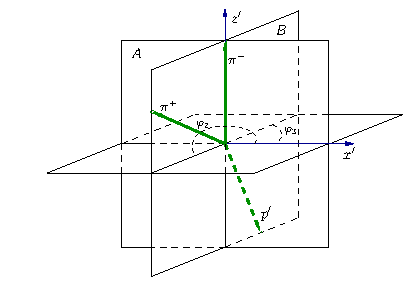
\includegraphics[width=12cm]{pictures/lab_mom_calc/ang_planes_gen.pdf}
\caption{\small Auxiliary frame CMS$'$ with the following axis orientation: $Z'$ -- along the first hadron and $X'$ -- perpendicular to $Z'$ and situated in the plane $A$. The plane $A$ is the plane, where the initial proton, virtual photon, and the first hadron are located, and $B$ is the plane, where all final hadrons are situated (the same planes $A$ and $B$ are shown in Fig.~\ref{fig:alpha_2nd_set}).  } \label{fig:ang_pl_gen}
\end{center}
\end{figure}


The spatial angles defined by Eq.~\eqref{eq:cms_prime_spat_ang} together with the energies and momentum magnitudes defined by Eq.~\eqref{eq:cms_prime_en_mom_mag} define completely the four-momenta of final hadrons in the auxiliary frame CMS$'$.

\item Once the four-momenta of the final hadrons are defined in the auxiliary coordinate system CMS$'$ shown in Fig.~\ref{fig:ang_pl_gen}, one can transform them into the coordinate system with the usual CMS-axis-orientation, where $Z_{cms}$ -- along the virtual photon, $X_{cms}$ -- in the electron scattering plane $(e,~e')$, and $Y_{cms}$ -- perpendicular to the $XZ$-plane. For that purpose two subsequent rotations should be made.

First, the $Z'$-axis of the auxiliary system in Fig.~\ref{fig:ang_pl_gen} is rotated with the generated angle $\theta_{h}$ in the plane $A$ to set  $Z'$-axis along the virtual photon. This rotation transforms the four-momentum as $P' = P\cdot R_{\theta}$, with 

\begin{equation}
R_{\theta}=\begin{pmatrix}
cos\theta_{h} &0  &-sin\theta_{h}  &0 \\ 
 0& 1 & 0 &0 \\ 
 sin\theta_{h} &0  &cos\theta_{h}  & 0\\ 
0 &0  & 0 &1 
\end{pmatrix}.
\end{equation}

After this rotation the $X'$-axis is still in the plane $A$.

Then one should rotate the $X'$-axis with the generated angle $\varphi_{h}$ in the $X'Y'$-plane (around the $Z'$-axis) to bring the $X'$-axis into the $(e,~e')$-plane. This rotation transforms the four-momentum as $P'' = P'\cdot R_{\varphi}$, with 

\begin{equation}
R_{\varphi} = \begin{pmatrix}
 cos\varphi_{h}& sin\varphi_{h} & 0 &0 \\ 
 -sin\varphi_{h}& cos\varphi_{h} &  0& 0\\ 
0 & 0 & 1 &0 \\ 
 0&  0&  0&1 
\end{pmatrix}.
\end{equation}


After that the final hadron four-momenta are defined in the CMS with the usual axis orientation. 


\item Now one can perform the boost from the CMS to the lab$'$ frame. The prime means that although the proton is at rest in this system, the axis orientation is still like in the CMS. The boost is given by $P''' = P''\cdot R_{boost}$, with 
\begin{equation}
R_{boost} = \begin{pmatrix}
1 &0  &0  &0 \\ 
0 &1  &0  &0 \\ 
 0&  0& \gamma  &\gamma \beta  \\ 
 0&  0& \gamma \beta  & \gamma 
\end{pmatrix}, \, \, \, \beta =\frac{\sqrt{\nu^2+Q^{2}}}{\nu+m_{p}}, \, \, \,  \textrm{and} \,\,\,   \gamma =\frac{1}{\sqrt{1-\beta ^{2}}},
\end{equation}
where $\nu$ is the energy of the virtual photon in the lab frame, which is defined in Eq.~\eqref{eq:el_in_lab}, and $\beta$ the magnitude and $z$-component of the three-vector $\overrightarrow{\beta}=(0,0,\beta)$.~\footnote[4]{
Note: if you use ROOT function .Boost the positive sign should be assigned to the $z$-component of $\beta$-vector, i.e. .Boost(0,0,$\beta$).}

After the boost the four-momenta of the final hadrons are defined in the lab$'$ frame, which has the CMS-like axis orientation.

\item The only thing left is to rotate the coordinate axes into the usual lab frame axis orientation.

\begin{figure}[htp]
\begin{center}
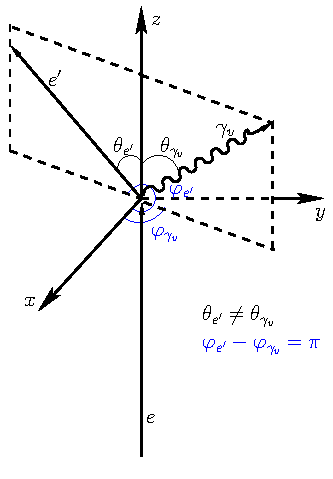
\includegraphics[width=6cm]{pictures/lab_mom_calc/electron_angles.pdf}
\caption{\small Virtual photon and scattered electron angles $\theta$ and $\varphi$ in the lab frame.} \label{fig:el_angles}
\end{center}
\end{figure}

For that purpose one firstly should define in the lab frame the vectors $\overrightarrow{n}_{e'}^{lab}$ and $\overrightarrow{n}_{\gamma}^{lab}$, which are the unit vectors along the scattered electron and virtual photon, respectively. The spatial angles of the scattered electron and virtual photon are shown in Fig.~\ref{fig:el_angles}. %They should be defined in the lab frame.

%We define the unit vector along the scattered electron in the lab-frame.
\begin{equation}
\overrightarrow{n}_{e'}^{lab} = sin\theta_{e'}cos\varphi_{e'}\overrightarrow{i} + sin\theta_{e'}sin\varphi_{e'}\overrightarrow{j} + cos\theta_{e'}\overrightarrow{k},
\end{equation}

where $\theta_{e'}$ is defined in Eq.~\eqref{eq:el_in_lab} and $\varphi_{e'}$ is the generated randomly value (see Sect.~\ref{sect:gen_with_weights}), $\overrightarrow{i}$, $\overrightarrow{j}$, $\overrightarrow{k}$ are the unit vectors along the $x$, $y$, $z$ axes of the lab system, respectively.

\begin{equation}
\begin{split}
\theta_{\gamma} &= acos \left ( \frac{Q^2+2E_{beam}\nu}{2E_{beam}\sqrt{Q^2+\nu^2}} \right )\\
\varphi_{\gamma} &= \begin{sqcases} 
\varphi_{e'} + \pi,\;\;if\;\varphi_{e'}<\pi \\ 
\varphi_{e'} - \pi,\;\;if\;\varphi_{e'}>\pi 
\end{sqcases}\\
\overrightarrow{n}_{\gamma}^{lab} &= sin\theta_{\gamma}cos\varphi_{\gamma}\overrightarrow{i} + sin\theta_{\gamma}sin\varphi_{\gamma}\overrightarrow{j} + cos\theta_{\gamma}\overrightarrow{k}.
\end{split}
\end{equation}


The idea of the coordinate system transformation is that the unit axis-vectors $\overrightarrow{u}$, $\overrightarrow{v}$, $\overrightarrow{w}$ of the system lab$'$ should be written in the lab system:

\begin{equation}
\begin{split}
\overrightarrow{w} &= \overrightarrow{n}_{\gamma}^{lab} = sin\theta_{\gamma}cos\varphi_{\gamma}\overrightarrow{i}+sin\theta_{\gamma}sin\varphi_{\gamma}\overrightarrow{j}+cos\theta_{\gamma}\overrightarrow{k}\\
\overrightarrow{v} &= [\overrightarrow{n}_{\gamma}^{lab}\times \overrightarrow{n}_{e'}^{lab}] = \begin{vmatrix}
\overrightarrow{i} & \overrightarrow{j} & \overrightarrow{k}\\ 
sin\theta_{\gamma}cos\varphi_{\gamma} & sin\theta_{\gamma}sin\varphi_{\gamma} & cos\theta_{\gamma}\\ 
sin\theta_{e'}cos\varphi_{e'} &sin\theta_{e'}sin\varphi_{e'}  &cos\theta_{e'} 
\end{vmatrix}\\
\overrightarrow{u} &= [\overrightarrow{v}\times \overrightarrow{w}].
\end{split}
\end{equation}

%where $\overrightarrow{u}$, $\overrightarrow{v}$, $\overrightarrow{w}$ are the unit vectors along the $x$, $y$, $z$ axes of the lab$'$ system, respectively.
\vspace{5em}
The four-momenta are transformed as $P'''' = P'''\cdot R_{lab}$~\footnote[5]{Using embedded ROOT functions, this transformation can be coded via Euler angles in the following way. \\ 
TRotation rot; \\
rot.SetXEulerAngles$( atan2\left (u_{z},v_{z} \right ),acos\left ( w_{z} \right ),atan2 \left (  w_{x},-w_{y} \right ) )$; \\
P.Transform(rot);
}, with
 
\begin{equation}
R_{lab} = \begin{pmatrix}
 u_{x}& u_{y} & u_{z} &0 \\ 
 v_{x}& v_{y} & v_{z} & 0\\ 
 w_{x}& w_{y} &  w_{z} &0 \\ 
 0&  0&  0&1 
\end{pmatrix}.
\end{equation}
\end{enumerate}


After all steps are completed the four-momenta of the final hadrons are written in the lab frame.
